% !TEX root = main.tex
\section{Theory}
\label{theory}

The PDIA posterior distribution takes the form of an infinite mixture of PDFAs.  In practice, we run a sampler for some number of iterations and approximate the posterior with a finite mixture of PDFAs.  We consider the expressive power of finite mixtures of PDFAs.  We find that they are strictly more expressive than PDFAs, but strictly less expressive than Hidden Markov Models.

The natural generalization of PDFAs is to probabilistic {\em non}-deterministic finite automata (PNFA), which are like PDFAs except the transition function $\delta$ is stochastic.  That is, given a state and a symbol emitted from that state, the next state is chosen from distribution over successor states.  If all successor state distributions assign mass to only one state, the PNFA is a PDFA.  PNFAs have the same expressive power as Hidden Markov Models, that is, for any HMM there is a PNFA that defines the same distribution over strings, and vice versa \cite{Dupont2005}.

PNFAs are a strictly larger model class than PDFAs.  For example, the simple PNFA in \ref{pnfa}(A) cannot be expressed as a PDFA.  However, it is clear that a mixture of two PDFAs, one with $Q = \{q_0,q_1,q_3\}$ and the other with $Q = \{q_0,q_2,q_3\}$, is equivalent to the above automata.  Thus mixtures of PDFAs are a strictly larger model class than PDFAs.  However, if we replace transitions to $q_3$ with transitions to $q_0$, as in \ref{pnfa}(B), there is no longer any equivalent finite mixture of PDFAs, since the nondeterministic branch from $q_0$ can be visited an arbitrary number of times.  

In general, any PNFA where the nondeterministic transitions can only be visited once can be expressed as a mixture of PDFAs.  This can be done by splitting a PNFA with $n$ possible values for $\delta(q_i,s_j)$ into $n$ PNFAs with deterministic $\delta(q_i,s_j)$, and repeating until all transitions are deterministic.  This includes the class of acyclic PNFAs as a trivial subset.  If there are any cycles that return to a state with nondeterministic transition, there is no equivalent finite mixture of PDFAs.

It is important to note that the algorithm presented here will not always discover the appropriate mixture of PDFAs if the data-generating mechanism is like that in \ref{pnfa}(A).  Our intent is to clarify where the class of models that includes our posterior estimate falls in the Chomsky hierarchy, rather than to make any claim as to what class of models can be efficiently learned.

\begin{figure}
\begin{center}
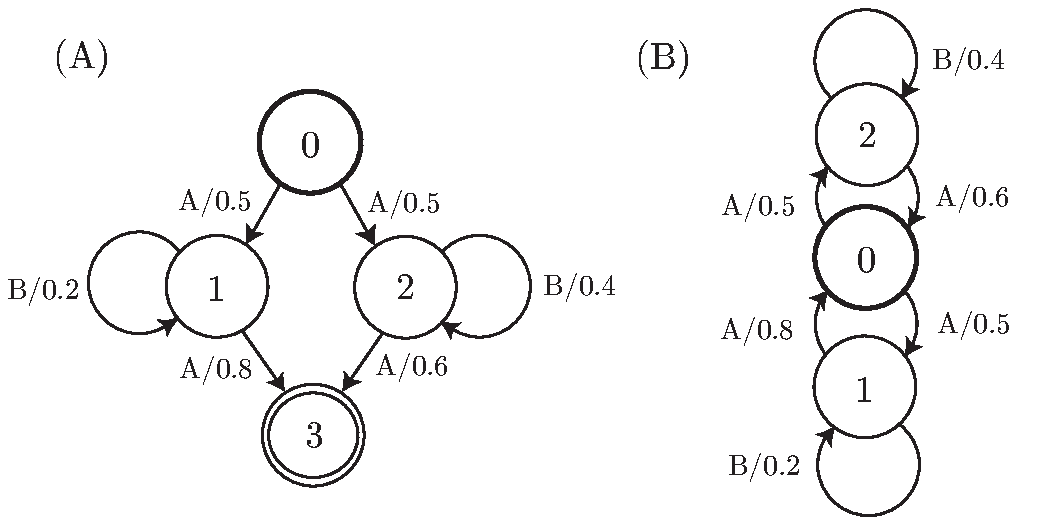
\includegraphics[scale=0.6]{pnfa.pdf}
\caption{Two PNFAs outside the class of PDFAs.  Automaton (A) can be represented by a mixture of two PDFAs, one following the right branch from state 0, the other following the left branch.  Automaton (B), in contrast, cannot be represented by any finite mixture of PDFAs, even though it is nearly the same as (A), but with transition to state 3 replaced by transitions to state 0.}
\label{pnfa}
\end{center}
\end{figure}